\chapter{Process overview}
 \label{cha:process_overview}
\todo[inline]{This is where the results are supposed to go, so there should be an introduction to them}
A detailed description of the dynamic model used in the present work can be found in \cite{Elisa_source}.
As a result, there will only a quick summary of the process will be given in this thesis. 

\section{Process overview}

\begin{figure}[htbp]
    \centering
    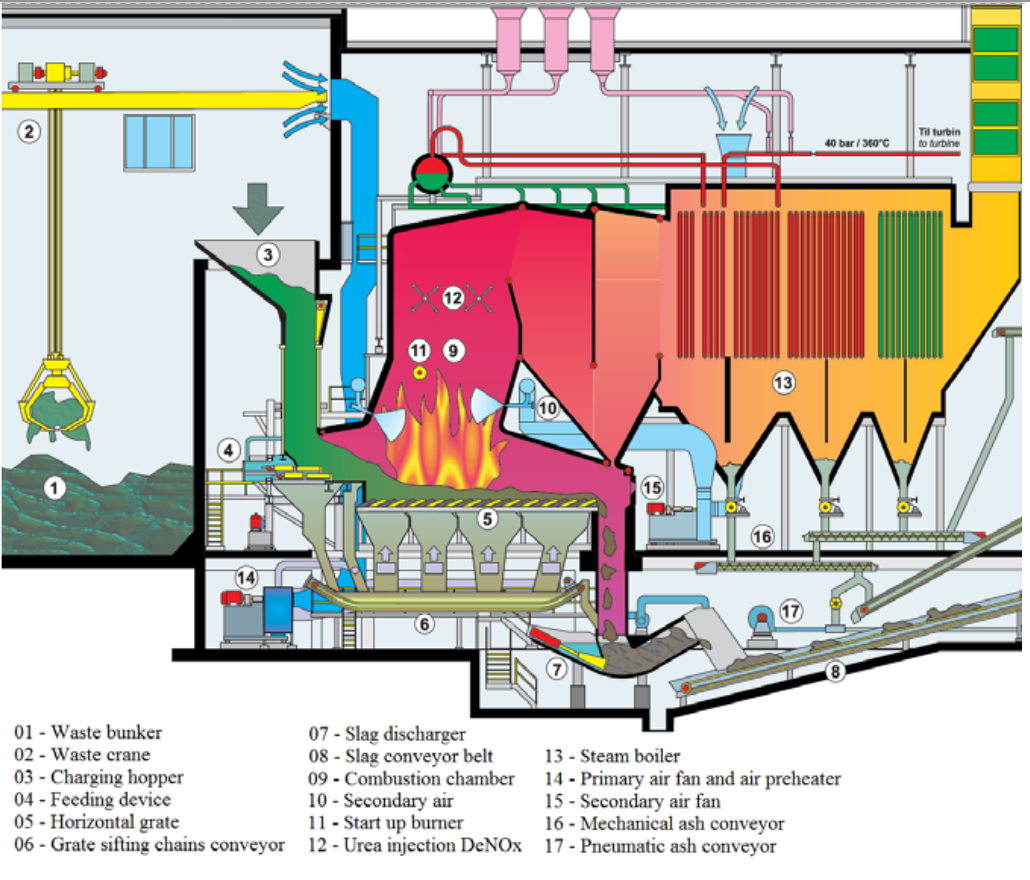
\includegraphics[width=\textwidth]{img/plant_overview.png}
    \caption{Overview of the plant}
    \label{fig:plant_overview}
  \end{figure}
  

As seen in Figure \ref{fig:plant_overview}, the waste is normally delivered to the waste-bunker (1). There, a set of cranes are used to mix it, to make it more homogeneous, decreasing how much the waste-composition varies, and therefore the disturbances. Some of it is then fed into the charging hopper (3) by the same cranes. A ram (4) pushes the waste onto the waste-grates (5). While on the grate, the primary air-flow (17) dries the waste and provides oxygen for the primary combustion. The conversion process taking place on the grates can be seen as divided into three sections. The waste is dried in the first section. On the second section of the grate, the primary combustion happens, where most of the heat is produced. The third part of the grate, any post-combustion happens to ensure that the amount of combustible material in the ash is below a certain threshold\footnote{In addition to the environmental damage that may come from exceeding these limits for too long, the limits are also enforced by law}. The non-combustible ash is then removed(17) from the system to be cleaned and disposed of. The combustion also results in the production of various gasses, which together with the air that did not react make up the  flue-gas. Somewhere above the second part of the grate, a secondary airflow is also applied to the volatile gases resulting from the primary combustion. This is where secondary combustion occurs, producing more heat through the further conversion of the gases produced by conversion on the grate (e.g. $CO$, $H_2$ and $CH_4$). The primary and secondary airflow(10) provide oxygen to the fire so that the combustion is complete. The two air-flows are added at two different points to allow for better mixing between flue gases and oxygen. Proper mixing is a requirement for having complete combustion and for reducing the formation of $NO_x$ and other harmful gases. The heat-exchange between the burning waste and the flue gas happens through contact, the mass-transfer of gases produced during combustion and by radiation. The flue gas in the combustion chamber(9) has a temperature of roughly $850^O C$. By law, the flue gas need to stay above $850^O C$ for at least 2 seconds. This is to ensure that no dangerous gases are produced. The flue gas travels through multiple bends, called passes. The passes make up the first section of the boiler (i.e. evaporator). The walls in the passes are made up of pipes where saturated water flows. When the gas flows past the pipes, it gives off heat to the walls, turning the saturated water  into saturated steam.  The second part of the boiler(13) (i.e. superheater) , is where the gas is used to heat a flow of saturated steam that is extracted from the boiler drum.  The final heat exchange section is called the economizer. Here, the cold water that is feed into the boiler drum is pre-heated to better take advantage of all the heat in the flue gas. Finally, the flue gas exits out of the system that is to be controlled in this thesis and into the part of the plant where it is cleaned before being released into the atmosphere. The composition of the flue gas that is released will depend on the amount of oxygen, how well oxygen and flue gas was mixed during combustion, the temperature in the combustion chamber, as well as the composition of the waste that is being burned. 
